\documentclass[a4paper]{article}

%% Language and font encodings
\usepackage[english]{babel}
\usepackage[utf8x]{inputenc}
\usepackage[T1]{fontenc}

%% Sets page size and margins
\usepackage[a4paper,top=3cm,bottom=2cm,left=3cm,right=3cm,marginparwidth=1.75cm]{geometry}

%% Useful packages
\usepackage{amsmath}
\usepackage{graphicx}
\usepackage[colorinlistoftodos]{todonotes}
\usepackage[colorlinks=true, allcolors=blue]{hyperref}

\usepackage[authoryear]{natbib}

%% My definition
\newcommand{\toshi}{\textcolor{blue}}
\newcommand{\laurie}{\textcolor{red}}
\newcommand{\rishi}{\textcolor{green}}
\newcommand{\iago}{\textcolor{purple}}

\newcommand{\disp}{\displaystyle}

\usepackage{enumitem}
\usepackage{algorithm}
\usepackage{algorithmicx}
\usepackage{algpseudocode}

\usepackage{color}
\definecolor{darkgreen}{rgb}{0.0, 0.5, 0.0}
\definecolor{darkred}{rgb}{0.7, 0.11, 0.11}
\definecolor{darkblue}{rgb}{0,0,0.5}
\definecolor{shadecolor}{rgb}{1,1,0.95}
\definecolor{shade}{rgb}{1,1,0.95}
\definecolor{coilin}{rgb}{1,0,1}

\title{Is It You or Your Model Talking}
\author{Laurence Kell, Toshihide Kitakado, Rishi Sharma, Henning Winker, \\ Iago Mosqueira, Dan Fu, Max Cardinale, ...}

\begin{document}


\section*{ICES Background}

Observational data are imperfect, and predictive models based on those data represent simplifications of how some aspect of the world works. Thus, in the fisheries advisory process (e.g., development of catch advice using stock assessments, evaluation of management strategies), it is clear that our analyses are fraught with uncertainty, stemming from uncertainty in the input data (observations) or from the \laurie{structure (degree of simplification and validity of assumptions)} of the methods and models employed. Input uncertainty is easier to measure using standard statistical procedures, and to address through improvements to survey designs, sampling schemes, and statistical methods. \laurie{Structural uncertainties however, are more intangible as they often represent “known unknowns” - i.e., we know there are limitations to the methods and models, but it is difficult to describe and measure them without comprehensive analyses, such as simulation testing or cross-validation}.

With the development of more advanced analytical frameworks that support implementation of  machine learning, artificial intelligence, and ensemble modeling, we invite fisheries scientists to a session to present advances in \laurie{identifying, quantifying and dealing with structural uncertainties in the fisheries science advisory process.}

We invite contributions on the following themes:

\begin{itemize}
    \item \laurie{Uncertainties throughout the stock assessment and management strategy evaluation process}
    \item \laurie{Identification and testing of plausible structural hypotheses, and structural uncertainties}
    \item \laurie{Sensitivity analysis}
    \item \laurie{Model ensembles (within and between models) see previous \href{ https://www.fisheries.noaa.gov/national/population-assessments/noaa-fisheries-13th-national-stock-assessment-workshop-report-released}{NOAA workshop} }
    \item \laurie{Gaps and needs for developing ensembles}
    \item \laurie{Evaluating trade-offs between one versus multiple models}
    \item \laurie{Combining and communicating results across ensemble members and stakeholders}
\end{itemize}


\maketitle
 
\section*{Still To Do}
\begin{itemize}
   \item Review sections in include files, make sure the text is complete, not redundant,  and fits into the overall text.
   \item Finalise results by adding tables if they help.
   \item Discussion based on elements that are in the outline.
   \item Mention process error \& recruitment patterns then do in Surplus Production paper  
   \item Get Max and Dan to review and submit to IJMS by June 30th
\end{itemize}

 \section*{Outline}
\begin{itemize}
    
    %\item The provision of fisheries management advice requires the assessment of stock status relative to reference points, the prediction of the response of a stock to management, and checking that predictions are consistent with reality (Holt pers com.) 
    
    %\item The Precautionary Approach requires the development of advice that is robust to uncertainty. Therefore, often when conducting stock assessments multiple models with different structures and datasets, are used to explore uncertainty. This means, however, that it is difficult to compare models using conventional metrics such as AIC. 
    
    \item  We  therefore compare SS, SS-ASPM, and Jabba assessments for Indian Ocean yellowfin tuna  using multiple metrics, and discuss hypothesis testing, model selection and model validation. We make recommendations for the bench-marking of stock assessment methods and discuss the consequences for MSE. In particular weighting of alternative Operating Models, modelling process error, and the development of Observation Error Models.   

    
   \item We therefore predict forward the retrospective analyses and compare model predictions with historical estimates.The absence of retrospective patterns, however, while reassuring is not sufficient as it is not possible to validate models based on model outputs. We therefore conduct model free hindcasts to compare observations with model estimates. 
   
   \item The use of metrics based on prediction skill allows different data components and model to be compared in order to explore data conflicts and potential model misspecification. The accuracy and precision of predictions depend on the validity of the model, the information in the data, and how far ahead predictions are required. 
    
\end{itemize}

\newpage
\tableofcontents 



\newpage    
\begin{abstract}
    Evaluating how well the model fits data has been receiving much attention in fisheries science, both in terms of goodness-of-fit and retrospectively. This however merely tells us how well we can describe the past, yet little how well we can predict the future under alternative management actions. In this paper, we revisit the concepts behind hindcasting cross-validation (hcxval) as an important model-free validation tool for predictive modelling. Together with conventional residual diagnostics and retrospective analysis, we apply hcxval to three examples of alternative candidate models using the recent Indian Ocean yellowfin tuna assessment as a case study. 
    These models comprise the 2019 spatially structured reference model implemented in Stock Synthesis (ss-ref), a deterministic age-structured production model (ss-aspm) of ss-ref and a simplied spatially aggregated stochastic surplus production model implemented in the 'JABBA' package. To assess prediction skill, we computed the Mean-Absolute-Scaled-Error (MASE), which, unlike e.g. Aikaike's Information Criterion, enables to compare across different models fitted to different data. The best MASE values (MASE < 1) were determined for ss-asem, which indicates that recruitment deviations in ss-ref were poorly estimated due to no or limited information in the 'noisy' length composition data. By contrast, the area effects retained in ss-aspm best explained its superior prediction skill compared to the spatially aggregated jabba model. We suggest that one-step ahead predictions are efficient for detecting overfitting and for model validation in general, but for future quota advice the forecast horizon should preferably at least match the assessment interval to ultimately increase confidence in the model-based scientific advice by stakeholders, managers and policy makers.
\end{abstract}

\newpage
\section{Introduction: Laurie + Toshi}

To provide fisheries management advice requires predicting the response of a stock to management and checking that the predictions are consistent with reality (pers. com. Sidney Holt). The accuracy and precision of predictions depend on the validity of the model, the information in the data, and how far ahead we wish to predict. The Precautionary Approach requires the development of advice that is robust to uncertainty. Therefore, when conducting stock assessments multiple models with different structures and datasets, are often used to explore uncertainty. 

In stock assessment, however, most goodness of fit diagnostic are either based on model residuals or retrospective analysis obtained from fits to historical observations. While the use of different modelling frameworks with different data needs means that it is difficult to select models using conventional metrics such as AIC.  As well as model selection which searches for the most suitable model within a family, and hypothesis testing which examines if the model structure can be reduced, model validation is also required. Validation examines if a model should be modified or extended and is complementary to model selection and hypothesis testing.

Model validation is important in many fields, e.g. in energy and climate models, as it increases confidence in the outputs of a model and leads to an increase in trust amongst the public, stake and asset-holders and policy makers \citep{kell2019optimising}. For models to be valid they must satisfy four prerequisites \cite{hodges1992you}: the situation being modelled must (i) be observable and measurable, (ii) it must be possible to collect sufficient data informative about it, (iii) exhibit constancy of structure in time, and (iv) exhibit constancy across variations in conditions not specified in the model. The first two prerequisites should be straight forward, but many stock assessments depend on fisheries dependent data rather than observation. For example highly migratory stocks fished in areas beyond national jurisdiction (ABNJ) commonly employ indices of abundance based on commercial catch rates. Prerequisite iii ensures that the model has predictive skill for the same conditions under which the validation tests were conducted, while prerequisite iv ensures that the model will still be valid for conditions that differ from those in the validation tests, i.e. can be used to set robust management advice. 

 We  therefore compare SS, SS-ASPM, and Jabba assessments for Indian Ocean yellowfin tuna  using multiple metrics, in order to help improve bench-marking of stock assessment methods.
 
    
\section{Material and Methods}

Retrospective analysis  \citep{hurtado2014looking} is commonly used to evaluate the stability of stock assessment estimates from alternative models. Observations are sequentially removed from the terminal year, the model is then refitted to the truncated series and the difference between between estimates from the full and truncated time-series compared using the relative error (RE, a measure of bias). The use of model based quantities, however, means that bias can not actually be quantified. A reduction in both RE and mean squared error (MSE, a measure of variance) can be achieved by shrinking terminal estimates towards recent historical values, at the expense of prediction skill. The absence of retrospective patterns, therefore, while reassuring is not sufficient for model validation.

Therefore to compare the different family of models we extend retrospective analysis to conduct a hindcast. Where a hindcast or a backtest is a way of testing a model based on past events by comparing outputs match with known results. We therefore extend retrospective analysis by adding an additional step of projecting over the truncated years. We then conduct a model-free hindcast \cite{kell2016xval} to estimate prediction skill, defined as any measure of accuracy of a forecasted value to the actual (i.e. observed) value that is not known by the model \citep{glickman2000glossary}. 

\subsection{Assessment Methods: Rishi}

There has been a recent trend in stock assessment toward the use of integrated analysis that combines several sources of data into a single model by a joint likelihood for the observed data \citep[e.g.][]{doubleday1976least,fournier1982general,maunder2013review}. Datasets include records of catches and landings, indices of abundance based on catch per unit (CPUE) and from research surveys, and length classes and ages compositions based on samples. A commonly used integrated assessment method is Stock Synthesis \citep[SS3,][]{methot2013stock} that can be configured in multiple ways, allowing for a large number of scenarios to be developed that reflect uncertainty.

\cite{Maunder2015} proposed an age-structured production model (ASPM) based on SS as a diagnostic of process dynamics. This evaluates whether the observed catches alone can explain trends in the index of abundance. Since if the ASPM is able to fit the indices of abundance that have good contrast then a production function is likely to exists (i.e. the dynamics are driven by density dependent processes), and the indices provide information about absolute abundance. If  there is not a good fit to the indices, then the catch data alone cannot explain the trends in the indices. This can have several causes: namely (i) stock dynamics are recruitment-driven, (ii) the stock has not yet declined to the point at which catch is a major factor influencing abundance; (iii) the indices of relative abundance are not proportional to abundance; or (iv) the base-case model is incorrectly specified.

In the later case this may indicate that the model structure is misspecified or the data are incorrect. The ASPM has been shown \citep{carvalho2017can} to be the best method for detecting misspecification of the key systems-modeled processes that control the shape of the production function. This is a problem since when conducting an integrated assessments many of the required parameters are difficult to estimate \citep[e.g.][]{lee2011m,lee2012steepness} and have to be fixed or priors used. An alternative is to use biomass dynamic models based on a production function, that requires the estimation and fixing of fewer parameters. An example is JABBA an open source package that presents a unifying, flexible framework for biomass dynamic modelling, runs quickly, and generates reproducible stock status estimates \citep{winker2018jabba}.

The main datasets were those used in the Indian Ocean Yellowfin Tuna Assessment. The main data are time series of total catch and four catch per unit effort (CPUE) indices. Spatial stratification of the Indian Ocean is by four regions (figure \ref{fig:map}). The black arrows represent the configuration of the movement parameterisation.  Density contours represent of the dispersal of tag releases (red) and subsequent recaptures from Indian Ocean Regional tuna tagging program. Green circles represent the distribution of catches from the longline fishery aggregated by 5 longitude * 5 latitude for 1980 – 2017 (max. = 133 770 t).


\iffalse
There has been a recent trend in stock assessment toward the use of integrated analysis that combines several sources of data into a single model by a joint likelihood for the observed data \citep[e.g.][]{doubleday1976least,fournier1982general,maunder2013review}.  Datasets include records of catches and landings, indices of abundance based on catch per unit (CPUE) and from research surveys, and length classes and ages compositions based on samples. 

A commonly used integrated assessment method is Stock Synthesis \citep[SS3,][]{methot2013stock} that can be configured in multiple ways. For example Maunder and Piner (2015) proposed an age-structured production model (ASPM) based on SS as a diagnostic of process dynamics. This diagnostic evaluates whether the observed catches alone (taken out of approximately the correct ages) can explain trends in the index of abundance. On the one hand, Maunder and Piner (2015) suggest that if the ASPM is able to fit well to the indices of abundance that have good contrast (i.e. those that have declining as well as increasing trends), the production function likely exists, and the indices will provide information about absolute abundance. On the other hand, the authors suggest that if there is not a good fit to the indices, then the catch data alone cannot explain the trajectories depicted in the indices of relative abundance. This can have several causes: (i) the stock is recruitment-driven; (ii) the stock has not yet declined to the point at which catch is a major factor influencing abundance; (iii) the base-case model is incorrect; or (iv) the indices of relative abundance are not proportional to abundance. Alternatively, failure in the ASPM may indicate a system that is not well organized (e.g., stock structures or data are incorrect) so that a real fishing signal is lost or where unknown environmental drivers control population abundance. The ASPM was shown via simulation analyses to be the only tested diagnostic capable of detecting misspecification of the key systems-modeled processes that control the shape of the production function \citep{carvalho2017can}.

A problem with integrated assessments is that many of the parameters required are difficult to estimate in practice \citep[e.g.][]{lee2011m,lee2012steepness} and have to be fixed or priors developed. An alternative is to use biomass dynamic models based on a surplus production function, that requires the estimation and fixing of fewer parameters. Once example is JABBA an open source package that presents a unifying, flexible framework for biomass dynamic modelling, runs quickly, and generates reproducible stock status estimates \citep{winker2018jabba}.
\fi


%\cite{maunder2006interpreting}
%\cite{langley2015yft}
%\cite{langely2016yft}
%\cite{langley2016yft2}
%\cite{urtizberea2018yft}




\subsection{Materials: Iago}
Yellowfin tuna (Thunnus albacares) supports one of the largest tuna fisheries in the Indian Ocean, with catches currently exceeding 400,000t, where they are harvested by a variety of gears, from small-scale artisanal fisheries, to large gillnetters, and industrial longliners and purse seiners \citep{fiorellato2019tt}

The stock is estimated to be overfished due to an increase in catch levels in recent years and consequently, IOTC introduced a rebuilding plan in 2016 to reduce the overall fishing pressure on the stock. Since 2015, the assessment of has been implemented using Stock Synthesis \citep[SS3][]{methot2013stock}. The SS3 assessment \citep[e.g.][]{\cite{urtizberea2018yft} implements an age and spatially structured model that reflected the complex population and fishery dynamics of the stock. Model development has focused primarily on determining an appropriate spatial structure that accounts for the differences in regional exploitation pattern and the level of tag mixing, incorporating seasonal movement dynamics, resolving data conflicts, and exploring non-stationary in selectivity and catchability.  

The most recent assessment \citep{fu2018yft} established a base case as a reference model for diagnostics along with scenarios that capture a range of uncertainties. The assessment indicated that stock  has declined substantially since 2012, and spawning stock biomass in 2017 is now estimated to be close to the historical lowest level. 

The base case is spatially dis-aggregated into two tropical regions that encompass the main year-round fisheries and two austral, subtropical regions where the longline fisheries occur more seasonally \citep{Langley2015}, with reciprocal movement assumed to occur between adjacent regions (Figure \ref{fig:map}). The model is based on a quarterly time step to approximate  continuous recruitment and rapid growth seen in the stock. Twenty-five fisheries were defined based on fishing gear, region, time period, fishing mode and vessel type. Most fisheries were modelled allowing flexiblity in selectivity (e.g. cubic spline or double normal), whereas long-line selectivity was constrained to be fully selective for the older fish.  The population comprised 28 quarterly age-classes with an assumed unexploited equilibrium initial state in each region. 

Recruitment occurs in the two equatorial regions with temporal deviates in the regional distribution and was assumed to follow a Beverton and Holt stock recruitment relationship (with a steepness of 0.8 and recruitment standard deviation of 0.6). 

Growth was parameterised using age-specific deviates on the k growth parameter to mimic the non-von Bertalanffy growth of juvenile and near linear growth of adults. 

Natural mortality is variable with age with the relative trend in age-specific natural mortality based on the values applied in the Pacific Ocean. 

The data used for fitting are catch and length composition data, longline CPUE indices, tagging recaptures, and environmental data. The length composition was weighted such that they were sufficient to provide reasonable estimates of fishery selectivity and recruitment trends but not directly influence the trends in stock abundance. Regional environmental indices (current and sea temperature) allows seasonal and temporal variations to be incorporated in the estimation of the fish movement. 

Tag release/recovery data collected from the main phase of the IO large-scale tuna tagging programme were integrated into the model to inform estimates of fishing mortality, abundance, and movement. 

The CPUE indices represent the primary source of information on abundance and is based on a composite longline index from the main distant water fleets \citep{Hoyle2018a}.
Indices in each region were standardised using generalized linear models that accounted for differences in targeting practices and catchablity amongst fleets, based on gear configurations and species composition. The reason for this is because tuna longline fishing strategies have changed over time \citep{Hampton2005}. In the assessment, the CPUE indices across regions were linked by a common catchability coefficient, thus improving the ability of the model to estimate the distribution of biomass by region \citep{Langley2015, Fu2018}. 

%%%%%%%%%%%%%%%%%%%%%%%%%%%%%%%%%%%%%%%%%%%%%%%%%%%%%%%%%%%%%%%%%%%%%%%%%%%%%%%%%%%%%%%%%%%%
%% Ignored after here %%%%%%%%%%%%%%%%%%%%%%%%%%%%%%%%%%%%%%%%%%%%%%%%%%%%%%%%%%%%%%%%%%%%%%
%%%%%%%%%%%%%%%%%%%%%%%%%%%%%%%%%%%%%%%%%%%%%%%%%%%%%%%%%%%%%%%%%%%%%%%%%%%%%%%%%%%%%%%%%%%%

\iffalse

Yellowfin tuna (Thunnus albacares) support one of the largest tuna fisheries in the Indian Ocean, where they are harvested with a variety of gear types, from small-scale artisanal fisheries, to large gillnetters, and industrial longliners and purse seiners, with current total catches over 400,000t \cite{fiorellato2019tt}

The stock is estimated to be overfished due to an increase in catch levels in recent years and consequently, IOTC introduced a rebuilding plan in 2016 to reduce the overall fishing pressure on the stock. Since 2015, the assessment of IO yellowfin tuna was implemented using the Stock Synthesis software (SS3) (Langley 2015, 2016, Fu et al. 2018, Urtizberea et ta. 2019). The SS3 assessment implements an age- and spatially structured model that reflected the complex population and fishery dynamics of the species. To date model development has focused on determining an appropriate spatial structure that accounts for the differences in regional exploitation pattern and the level of tag mixing, incorporating seasonal movement dynamics, resolving data conflicts, and exploring non-stationary processes (e.g. selectivity and catchability).  The most recent benchmark assessment \cite{fu2018yft} has established a model ensemble to capture a range of uncertainties and adopted a reference case for diagnostics purposes (IOTC 2018). The assessment indicated stock biomass declined substantially since 2012, with the spawning biomass in 2017 estimated to be close to the historically low level. We use the reference model as the test case in the paper which is briefly summarized as below.  More details of the model specification are in in \cite{fu2018yft}.

The reference model is spatially disaggregated into two tropical regions that encompass the main year-round fisheries and two austral, subtropical regions where the longline fisheries occur more seasonally (Langley 2015), with reciprocal movement assumed to occur between adjacent regions (Figure 1).  The time period (1950 – 2017) were compiled into quarters (defined to be model “years”) to approximate the continuous recruitment and rapid growth. Twenty-five fisheries were defined based on fishing gear, region, time period, fishing mode and vessel type. Most fisheries used a flexible selectivity form (e.g. cubic spline or double normal) whereas the longline selectivity was constrained to be fully selective for the older fish.  The population is comprised of 28 quarterly age-classes with an unexploited, equilibrium initial state in each region. Recruitment occurs in the two equatorial regions with temporal deviates in the regional distribution and was assumed to follow a BH stock recruitment relationship (steepness of 0.8 and sigmaR of 0.6). The growth was parameterised using age-specific deviates on the k growth parameter to mimic the non-von Bertalanffy growth of juvenile and near linear growth of adults. Natural mortality is variable with age with the relative trend in age-specific natural mortality based on the values applied in the Pacific Ocean.  The data fitted in the model consist of catch and length composition data, longline CPUE indices, tagging recaptures, and environmental data. The length composition was weighted such that they were sufficient to provide reasonable estimates of fishery selectivity and recruitment trends but not directly influence the trends in stock abundance. Regional environmental indices (current and sea temperature) allows seasonal and temporal variations to be incorporated in the estimation of the fish movement. Tag release/recovery data collected from the main phase of the IO large-scale tuna tagging programme were integrated into the model to inform estimates of fishing mortality, abundance, and movement. 

The CPUE indices represent the primary source of information on abundance and was based on a composite longline catch effort data from main distant water longline fleets standarised in a unified framework (Hoyle et al. 2018a). The Joint standardization utilized substantive logbook programmes with extensive history and broad sampling coverage and is considered a better approach than using fleet-specific, potentially conflicting indices. A data filter was used to indenfity credible data subsets to mininimze the conficts of trend amongst fleets which are thought to be mainly caused by lower spatial coverage or missiporting from fleets (Hoyle et al. 2018b). Indices in each region were standardised using generalized linear models that accounted for differences in targeting practices and catchablity amongst fleets, based on gear configurations and species composisiton (in areas with known distinctive targeting behaviour). This is important as tuna longline in all oceans is known to have changed fishing strategies over time (Hampton et al. 2005). In the assessment model, the respective CPUE indices among regions were linked by a common catchability coefficient, thus improving the ability of the model to estimate the distribution of biomass among regions (Langley 2015, Fu et al. 2018). As such the regional indices were scaled by the respective regional scaling factor which incorporated both the size of the region and the catch rate to index the relative level of exploitable long-line biomass among region (Hoyle and Langley 2020). Temporal trends in the standardized indices vary within regions, with greater decline in CPUE in tropical areas close to the equator (Figure 2). The trend does not appear to be consistent with the general perception of the high degree of mixing of the populations between regions 1 and 2 as induced by oceanographic conditions but may have been associated with greater depletion of areas subject to more purse seine fishing (Hoyle et al. 2018b).  It is also possible that the recent steeper decline of CPUE indices in region 1 could be reflective of fishing operation and/or a change in the fleet composition rather than abundance (Fu et al 2018).  In addition, the exceptionally high peak in CPUE indices the late 1970s is most likely associated with reporting and data management (Hoyle et al 2017), and the spike around 2012 in region 1 may have reflected changes in the population or catchability as vessels returned to areas once affected by piracy. 

\fi



\subsection{Hindcast: Laurie then Henning}

Hindcasting like traditional retrospective analysis involves fitting a model using a tailcutting procedure, where data are deleted sequentially for $n$ years, i.e. from the last year $y$ through to $y−n$, the additional step in the hindcast is that then the data from year 1 to $y−n−1$ are used to make predictions of what will happen in years $y−n$ to $y$.

\begin{algorithm}[!ht]
\begin{algorithmic}[1]

\State Conduct assessment for all years, i.e. $t=n$
\For ~ $t$ = n to n-20
\State Remove all $X_{i,t}$ for $t$ to n
\State Run model
\State Estimate $\hat{X}_{i,t}$ to $\hat{X}_{i,n}$ 
\EndFor
\caption{Hindcast~\citep{kell2016xval}}
\label{Hindcast}
\end{algorithmic}
\end{algorithm}

Hindcasting can be performed for model based quantities (e.g. SSB and F) or model-free (e.g. observations of CPUE). The former helps check the stability of stock assessment advice, while the later provides an objective way to validate models based on prediction skill and to test for over-fitting. The later is important since analysis of residuals is a common way to determine a model’s goodness-of-fit \citep{Cox1968general}, since  non-random patterns in the residuals may indicate model misspecification, serial correlation in sampling/observation error, or heteroscedasticity. When inspecting residuals, however, there is a danger of hypothesis fishing, i.e. choosing a scenario retrospectively retrospect, while if multiple true hypotheses are tested it is likely that some of them will be rejected. Therefore it is valuable to reserve part of the data for validation, so that a pattern’s significance is not tested on the same data set which suggested the pattern \citep{thygesen2017validation}. For this reason we conduct a model-free hindcast.

Since assessment cycles are typically for three years  with advice \citep{fricker2013three} we projected the truncated estimates for 3 years. When conducting the hindcast it is assumed that modelled variables are observable, processes exhibit constancy of structure in time, including those not specified in the model, and that collection of accurate and sufficient data is possible \citep{hodges1992you}.

\subsubsection{Model-Based}
A standard diagnostic is to evaluate retrospective bias as proposed by \cite{mohn1999retrospectyive}. As described in earlier sections, the retrospective analysis can be conducted by sequentially refitting the model to reduced data sets by removing some recent years' data to see if there are any systematic pattern within a model. The retrospective bias is then evaluated using the so-called Mohn's rho as 

\[
\rho = \disp \sum_{t=T-n}^{T-1} \frac{\hat{y}_{(1:t),t}-\hat{y}_{(1:T),t}}{\hat{y}_{(1:T),t}}, 
\]
where $\hat{y}$ denotes in general a value like estimated biomass, 1+population size, or predicted abundance index, and the value with suffix $\hat{y}_{(1:t^\prime),t}$ means such a value estimated at time $t$ of a full series from 1 to $T$ using a retrospective data window from 1 to $t^\prime (\leq T)$. In this paper, we will use a variant of the original $\rho$ as the mean (average) like 
\begin{equation}
\rho_r = \disp \frac{1}{n} \sum_{t=T-n}^{T-1} \frac{\hat{y}_{(1:t),t}-\hat{y}_{(1:T),t}}{\hat{y}_{(1:T),t}} 
\quad \mbox{[rho for retro-bias]}, 
\end{equation}
This metric is an average of relative differences at the final time of each window. Therefore it is a measure of relative retrospective `bias' (scale-free) in a statistical sense. The metric tends to be applied not on the log but the original scale because both the directions of positive and negative biases are regarded as being equivalent. 

While it is fairly straightforward to compare the  statistic among alternative model runs, the decisions of whether the Mohn’s $\rho$ statistic of the ‘best’ model is acceptable or not can be to some extent subjective. To address this, a “rule of thumb” was proposed by \cite{hurtado2014}, suggesting values of Mohn’s $\rho$ that fall outside the range (-0.15 to 0.20) can be interpreted as an indication of an undesirable retrospective pattern for e.g. longer lived species.


\subsubsection{Model-Free}
\vspace{0.2cm} \noindent
{\it Mean absolute scaled error (MASE) for projection:}\\ 
A robust and easier to interpret statistic for evaluating prediction skill is the MASE \citep{hyndman2006another}. MASE evaluates a model's prediction skill relative to a na\" {i}ve baseline prediction, based on previous observation. A prediction is said to have skill if it improves the model forecast compared to the baseline. A widely used baseline forecast for time series is the persistence algorithm that takes the value at the previous time step to predict the expected outcome at the next time step as a na\ "{i}ve in-sample prediction, i.e. tomorrow will be the same as today. The original definition of MASE for 1-step ahead perdition is 
\begin{equation}
{MASE=\frac{\disp \frac{1}{n} \sum_{t=T-n}^{T-1} \left| \hat{y}_{(1:t),t+1}-y_{t+1} \right|}
{\disp \frac{1}{n-1} \sum_{t=T-n+1}^{T-1} \left|y_{t+1}-y_{t}\right|}}, 
\end{equation}
and this can be extended as \red{actually not very much straightforward but seems as below}
\begin{equation}
MASE=
\frac{\disp \frac{1}{n-S+1} \sum_{t=T-n}^{T-S}  \left| \hat{y}_{(1:t),t+S}-y_{t+S} \right|}
{\disp \frac{1}{n-S} \sum_{t=T-n+1}^{T-S} \left|y_{t+S}-y_{t}\right|}. 
\end{equation} 

The MASE has the desirable properties of scale invariance, predictable behaviour, symmetry, interpretability and asymptotic normality. Compared to MAPE, which relies on the division by observations for scaling, MASE does not necessarily skew its distribution even when the observed values are close to zero. MASE is also easier to interpret as a score of 0.5 indicates that the model forecasts are twice as accurate as a na\''{i}ve baseline prediction; the model thus has prediction skill.
\vspace{0.2cm}

The best statistical measure to use depends on the objectives of the analysis and using more than one measure can be helpful in providing insight into the nature of observation and process error structures. Here for the evaluation of models, we use the following metrics: 
\begin{itemize}
\item Original Mohn's rho ($\rho$) for checking the retrospective bias \\
\vspace{-0.3cm}
\item Modified Mohn's rho for prediction \red{bias and absolute error, which? both might be meaningful though but it becomes noisy...} as checking model-based self-consistency check \\
\vspace{-0.3cm}
\item MASE and RMSE for model-free validation with different angles. 
\end{itemize}




\section{Results: Rishi}

The retrospective analysis for one and three step ahead prediction is shown in figure \ref{fig:retro} for $SSB:B_{MSY}$ and $F:F_{MSY}$ (SSB & F for SS and ASPM and exploitable biomass and harvest rate for JABBA). Even for a one year ahead prediction, the base case and JABBA assessments start to diverge from the assessment that included all years. The pattern gets worse for the three year projections. Table \tref{tab:retro} shows the estimates of Monh's $\rho$, RMSE, and MASE. This allows bias, variance and model-based prediction skill to be compared.

ASPM values are relatively unbiased with low variance and good prediction skill. For SS, however, there is over and underestimation of SSB and F respectively. For JABBA a strong negative retrospective pattern is seen in F, a negative bias is also seen in biomass.

The residuals from the model fits to the indices of abundance are shown in Figure~\ref{fig:runs}, the background indicates whether they passed (green) or failed (red) the runs tests. In general the CPUE for Area 2 and Area 4 perform poorly for both the base case and the JABBA models. 1st quarter indices also perform poorly compared to the other quarters (quarter 3 for CPUE 1 is also poorly predicted). As indicated the green shows that the runs test passes for most of the ASPM model data, and a lot more red indicators exist for the other two models.  

The results from the model-free hindcasts are shown in Figures~\ref{fig:hy} and \ref{fig:hy3} for one and three year ahead predictions respectively. CPUE's from area 2 and 4 perform poorly as in the previous figures for the base case and JABBA. The ASPM also performs poorly for Area 2 in the 3 year hindcast projections. Model fits for 3 years ahead for both JABBA and the base case perform poorly. Area 2 also fails for ASPM in the 3 year projections. As a bulk of the catch comes from Area 1 and 2, Area 2 index of abundance is important to predict. In addition Area 4 in the eastern part of the Indian Ocean perform poorly with all models in the three year hindcast exercise.   

The fits are summarised in Figures~\ref{fig:td} in the form of Taylor diagrams \citep{taylor2001summarizing}. 

%In the one year hindcast, all models other than area 2 indices had a high RMSE, high sigma, and low correlation (left panel). Other models seem to have a high overlap (lower left cluster indicating a high correlation, and low RMSE and low sigma). As we go to a three year hindcast, all models seem to perform poorly, other than the ASPM. Even, the ASPM, appears to do poorly with the 2nd CPUE. the correlation gets worse for all models for CPUE 1 & 2, though the RMSE and sigma remains low.  

Table \ref{tab:retro} and  \ref{tab:proj} show Mohn's $\rho$ for the retrospective analysis and retrospective with projection, Table \label{tab:rmse} shows the values of RMSE and \label{tab:mase} MASE for the model free hindcast.

\begin{description}
    \item{Retrospective analysis for F/FMSY and B/BMSY}
  
    \begin{itemize}
        \item Figure \ref{fig:retro} and Table \ref{tab:retro} summarise the retrospective analysis, taking 0.2 and -0.15 as the cut off points for accepting an assessment all assessments pass. 
        \item The strongest retrospective patterns are seen for SS, where F is negatively biased, and although the value of Mohn's $\rho$ is low for SSB a strong pattern is seen with underestimates followed by overestimates. 
        \item Although recent Jabba estimates are unbiased historical estimates of F and Biomass are negatively biased.
        \item Jabba estimates are problematic as it appears that even if F<FMSY the stock will decline below BMSY
        \item ASPM estimates appears to have little bias
    \end{itemize}
    \item{Retrospective analysis and projections for F/FMSY and B/BMSY} 
    \begin{itemize}
      \item Figure \ref{fig:proj} and Table \ref{tab:proj} summarise the retrospective analysis combinded with a three prediction, again taking the cut off as 0.2 to -0.15, both SS and Jabba fail.
      \item ASPM appears not to show patterns in the projections
        \item ASPM performs best
        \item Survey 2 performs poorly across all models
        \item It appears that the length compositions add noise (SS), and that area effects (JABBA) are important.
        \item However these is no objective way to choose an assessment based on retrospective analysis as the best model would always be B/MSY = 1 
   \end{itemize}
   \item{Residuals}
    \begin{itemize}
        \item Figure \ref{fig:runs} summarises the residuals, in the form of runs test; green backgrounds denote a pass. Only two indices pass for all models Survey 1 quarter 1 and Survey 3 quarter 4
        \item Over half of the indices fail for Jabba, half for SS while for ASPM the majority pass. This indicates strong data conflicts while  failure of the runs test may explain the retrospective patterns.
   \end{itemize}
     \item{Model-free cross-validation} confirms the relative performance of the models
    \begin{itemize}
        \item Figures \ref{fig:hy1} and \ref{fig:hy3} shows that SS performs poorly, possibly because length compositions can only be explained by variations in year-class strengths, and projections predict large increase in biomass.
        \item RMSE is difficult to interpret (Table \ref{tab:rmse}), MASE easier (Table \ref{tab:mase}).
        \item Taylor diagram, shows that there is a big difference between model residuals and prediction residuals. Figure \ref{fig:td} summarises the historical model fits survey 4 performs the best, i.e. has high correlation for all models, while survey 3 performs poorly.
        \item However, when three step ahead projections are considered (Figure \ref{fig:tdhat} ) survey 4 perform the best for ASPM, although the correlation is reduced. SS has high RMSE, poor correlation and high  variance.  
   \end{itemize}
 \end{description}

\section{Discussion: All}
\section{Discussion}

What we did
[I think the discussion need to be shortened and reorganised a bit. Suggest firstly focusing on the technical aspects of  hincasting, with reference to YFT application, then discussing its merits/advantages over other methods - likelihood-based approach and retrospective analysis, and then progress to the discussion of using this approach to help determine the selection of model grid, with reference to ICCAT applications, and then touch upon other topics such as such as model weighting, with reference to MSE].
]

[I think there need to be some general comments/comparisons on the three models analysed, suggested something like:

There is often trade-off in explanatory and predictive powers amongst models with varying levels of complexity. Highly parameterised, disaggregated models tend to have to a high degree of explanatory power as they are capable of describing a wide range biological and population processes. But such models often has a high degree of estimation variance resulting in poor predictive capability when there is insufficient data to estimate the underlying biological drivers, 
On the other hand relatively simple models (e.g. deterministic production models) may lack the explanatory power to describe the dynamics in sufficient details, but their simple structure can be better characterised by the available data, leading to increased precision in model predictions.

]

\begin{itemize}
    \item  We  compared SS, SS-ASPM, and JABBA assessments for Indian Ocean yellowfin tuna  using prediction skill, and discuss hypothesis testing, model selection and model validation. We make recommendations for the bench-marking of stock assessment methods and discuss the consequences for MSE. In particular the selection of stock assessment scenarios, the weighting of alternative Operating Models, modelling process error, and the development of Observation Error Models.   

   \item We used forward traditional retrospective analyses in order to compare model predictions with historical estimates. The absence of retrospective patterns, however, while reassuring, is not sufficient as it is not possible to validate models based on model outputs. We therefore conduct also model-free hindcasts (i.e. based on observable quantities as CPUE) to compare observations with model estimates. 
   
   \item The use of metrics based on prediction skill allows different data components and model to be compared in order to explore data conflicts and potential model misspecification. The accuracy and precision of predictions depend on the validity of the model, the information in the data, and how far ahead predictions are required. 
   
   \item The main objectives of management frameworks are to achieve management targets (e.g. $B_{MSY}$) and avoid limits (e.g. Blim) with high probability. Therefore stock assessments need to provide estimates of uncertainty when reporting stock status and forecast. These may be based on estimation error, e.g.  by bootstrapping a best assessment, or by the use of multiple models to represent model and parameter uncertainty or by the combination of both. 

  \item A best assessment is usually selected using AIC to find the most parsimonious model from within a set of scenarios. The use of AIC, however, means that multiple models with alternative datasets can not be evaluated. The use of the hindcast showed that the base case did not have prediction skill and that area effects were important, these results could not have been obtained at using AIC.\red{Should we mention here the cookbook philosophy? AIC is generally used but a more appropriate approach is via multiple diagnostics} 

  \item In some cases, e.g. ICCAT, multiple model families are used to conduct the assessment and then various methods used to generate uncertainty (e.g. bootstrap, MCMC, MVLN) in order to construct the Kobe Phase Plot. Without the use of a pre-agreed model validation procedure, however, it is difficult to either weight or reject models. Therefore, a key step in benchmarking is the procedure and criteria used to include models in the original grid. 

  \item An approach that has been proposed is ensemble modelling. The problems here is how to agree the scenarios to include and the weighting and acceptance criteria. Furthermore weighting of grids is only really possible if you use a common modelling framework like SS. In most if not all cases, however, the problems are unknown parameter values and data weighting. In which case the best approach is to develop robust management procedures. There is a need therefore to develop OMs based on hypotheses we can resolve, i.e. show the value of information. In the mean time we need to develop robust MPs based on the value of control \red{what do you mean here?}.
\end{itemize}
  
 What we think
 
\begin{itemize}
    \item An assessment model can not be chosen based on a retrospective analysis alone, since you can only validate a model using observations. For example a strong retrospective pattern can be improved using shrinkage \parencite{dickey2007precisely}. Such a model, however, would have little prediction skill if shrinkage simply removes recent year-class signals and changes in selection pattern, both of which determine future stock biomass and fishing mortality. Furthermore, in statistics shrinkage is used to reduce variance at the expense of increasing bias, however, using model outputs means that bias can not be estimated. 
    
    \item  While the retrospective-hindcast provides a useful diagnostic to check for consistency between predictions and historical model estimates, the use of latent state variable such as $B_{t}$ does not permit formal model validation. 

    \item Most goodness of fit diagnostics in stock assessment are based on the inspection of model residuals, obtained from fits to historical data, to identify patterns due to bias, drift, skewness, heavy tails, correlation with states or driving inputs, and heteroscedasticity.  It is rarely possible to conceive a list of tests on residuals before seeing them, which means that the hypotheses we are testing, implicitly or explicitly, are not proposed independently of data. There is therefore a danger of hypothesis fishing. Furthermore, if multiple true hypotheses are tested it is likely that some of them will be rejected incorrectly. This is not in agreement with the principles of statistics and is a well-known problem of post-hoc analysis. For that reason the ubiquitous significance level of 5\% should not be used uncritically \cite{wasserstein2016asa}. It is therefore good practice to reserve part of the data for validation, so that a pattern’s significance is not tested on the same data set which suggested the pattern.
    
    \item  The model-free hindcast provides an way to validate models based on prediction skill, since if MASE >1 then a random walk is better than the model. The MASE also allows you to compare across models and data series you how good the prediction skill is, since an a MASE of 0.5 is twice as good as a MASE of 1.  
    
    \item When MASE>1 this is probably because there are some processes that are not being modelled correctly or else the data series do not contain information on stock abundance or are in conflict with those where MASE<1. Therefore there is a need to extend or revisit the model structure. Since MASE can also be used to compare across models, unlike AIC, it can still be used in this process to compare new models and datasets. 
    
    \item Individual indices could also have been removed 1 year-at-time. The retrospective-hindcast, however is an important first step as it shows the transition from retrospective analysis of model based quanties (i.e. F and SSB) to the model-free hindcast.  Index by index model-free validation allows for direct inference about the impact of each index to be evaluated, which is important if we want to work out how to extend/modify the model.     

    \item  In the case of the YFT example, if only a retrospective analysis had been conducted and model residuals examined it may have been concluded that all models were equally good. By performing a 1 and 3 step ahead prediction, it was shown that the base case was modelling noise and JABBA by not accounting for spatial structuring has limited prediction skill. The best MASE values were seen for ASPM, since the length compositions were only added noise and area effects were important but were not included in JABBA.

    \item  The results have direct applications for developing a objective process to assign weights to candidate models within a model ensemble that included different families and datasets, and important in contrast to model selection and hypothesis testing, which are mainly used to reject models provides a procedure for future model development. For example to explore the importance of different processes.\red{something is missing here}

    %\item  Emphasize that these results are case specific and should not be generalized. What can be generalized is the here presented analysis, given than it is transferable across both platforms can be applied model scenarios that are fitted different data sets.

    \item The results have consequences for MSE, both for selection of OMs  which are used to simulate future states under feedback control, and the choice of indices to simulate in the OEM. If the SS base case has poor prediction skill how can it be used as the basis of OM development? The OEM generates data for use in the MP, the TDs characterise the process and measurement error, i.e. only indices with high correlation should be used as input to the MP. What if more than 1 OM scenarios has been conditioned with alternative data weightings and in each case there is a different preferred index? 

\end{itemize}


\section{Conclusions: All}

Primary objectives were:
\begin{enumerate}
    \item In fisheries unlike other fields we try to account for the past but not for the future. Here we propose a way to assess model predictive performance and to account for alternative models within a common diagnostic framework.  
    \item Unifying platform for evaluating across models
    \item Advantage of MASE : What are the new properties of this stat
    \item Consequences for stock assessment benchmarking
    \item Consequences for uncertainty, risk and MSE.
    \item Next steps
\end{enumerate}

\section{Appendix: Summary Metrics}
Indices of abundance are a key contributor to the overall likelihood when fitting stock assessment models to data. The Sum of Squared Errors (SSE) between observed and predicted indices in log-space is the measure of fitness. When comparing models, however, the SSE is problematic because complex models tend to have many parameters to allow flexibility when fitting, which may result in a low SSE due to overfitting. Therefore, information criteria, such as AIC, have been developed to aid in model selection. AIC is only a relative measure of the appropriateness of models, and additional diagnostic tests are required for model validation. This is of particular importance for stock assessment models where only a single historical data set exists, and the system can not be observed directly.

Therefore in stock assessment, a standard diagnostic is to evaluate retrospective bias as proposed by \cite{mohn1999retrospectyive}. As described in earlier sections, the retrospective analysis can be conducted by sequentially refitting the model to reduced data sets by removing some recent years' data to see if there are any systematic pattern within a model. The retrospective bias is then evaluated using the so-called Mohn's rho as 

\begin{equation}
\label{eqn:mohn0}
\rho_M = \disp \sum_{t=T-n}^{T-1} \frac{\hat{y}_{(1:t),t}-\hat{y}_{(1:T),t}}{\hat{y}_{(1:T),t}}, 
\end{equation}

where $\hat{y}$ denotes in general a value like estimated biomass, 1+population size, or predicted abundance index, and the value with suffix $\hat{y}_{(1:t^\prime),t}$ means such a value estimated at time $t$ of a full series from 1 to $T$ using a retrospective data window from 1 to $t^\prime (\leq T)$. In this paper, we will use a variant of the original $\rho$ as the mean (average) like 
\begin{equation}
\label{eqn:mohn}
\rho_{Mr} = \disp \frac{1}{n} \sum_{t=T-n}^{T-1} \frac{\hat{y}_{(1:t),t}-\hat{y}_{(1:T),t}}{\hat{y}_{(1:T),t}} 
\quad \mbox{[rho for retro-bias]}, 
\end{equation}
This metric is an average of relative differences at the final time of each window. Therefore it is a measure of relative retrospective `bias' (scale-free) in a statistical sense. The metric tends to be applied not on the log but the original scale because both the directions of positive and negative biases are regarded as being equivalent. 

Hindcasting, which is the primary focus in this paper is a form of retrospective cross-validation, and therefore an extension of retrospective analysis which projects several steps forward beyond the retrospective data window to quantify the prediction skill of a model. Theoretically, the projection period is to the end of the historical time period. However, in practice, the step size is one or several years ahead reflecting the requirements for robust management advice, and considering non-small process stochasticity in fishery population dynamics and non-ignorable extents of observation uncertainty. For evaluating prediction skill, we propose several metrics for model-dependent and model-free validations.

We  define `retro-period' and `hc-period' as `the period of shrunken data set for retrospective model fitting' and `future time period with a certain projection step (say $S \geq 1$) for hindcasting after retro-period''. And let $\hat{y}_{(1:t),t+S}$ be an projected value at time $t+S$ in an hc-period based on the conditioned model with data in a retro-period $(1,t)$. 

\vspace{0.2cm} \noindent
{\it Modified Mohn's rho for prediction bias and absolute error:}\\
\begin{equation}
\label{eqn:mohn2}
\rho_p = \disp \frac{1}{n-S+1} \sum_{t=T-n}^{T-S} 
\frac{\hat{y}_{(1:t),t+S}-\hat{y}_{(1:T),t+S}}{\hat{y}_{(1:T),t+S}} 
\ \mbox{[rho for projection-bias]}
\end{equation} 

This is a simple extension of Mohn's rho to evaluate the prediction skill of a model because all the values are produced under the model assumption. In this sense, it is a model-dependent consistency check of prediction skill. To evaluate the absolute prediction error for the following can be used
\begin{equation}
\label{eqn:mohn3}
|\rho_p| = \disp \frac{1}{(n-S+1)} \sum_{t=T-n}^{T-S}
\frac{\left| \hat{y}_{(1:t),t+S}-\hat{y}_{(1:T),t+S} \right|}{\hat{y}_{(1:T),t+S}}. 
\ \mbox{[rho for projection-absolute-error]}
\end{equation} 

There are problems with the use of relative error, since for reference model estimates which are low relative to the alternative model, i.e. $X_{ref} < X_{p}$, there is no upper limit, while for $X_{ref} > X_{p}$ the error cannot exceed 1.0. Therefore the chosen metric puts a heavier penalty on negative than on positive errors, i.e. historical underestimates. This means that when comparing models estimates, those that are low will be preferred. This problem can be overcome by using the logarithm of the ratio instead i.e. 
\begin{equation}
\label{eqn:re}
log\frac{X_{p}}{X_{ref}}
\end{equation}

which also leads to better statistical properties.


\vspace{0.2cm} 
The next three metrics are used for model-free validation, i.e. comparing predictions with observations. The error is defined as the difference between the predicted ($\hat{y}_{(1:t),t+S}$) and observed $y_{t+S}$) values, such as the model-based predicted CPUE using a retro-period data and observed CPUE used for model fitting. 

\vspace{0.2cm} \noindent
{\it Mean Absolute Percentage Error (MAPE) for projection:}
\begin{equation}
\label{eqn:mape}
MAPE = \disp \frac{1}{n-S+1} \sum_{t=T-n}^{T-S}
\frac{\left| \hat{y}_{(1:t),t+S}-y_{t+S} \right|}{y_{t+S}} \times 100 
\end{equation} 
A simple extension of the modified Mohn's rho for quantifying the relative difference between predictions and observations. This metric is also a scaled version of Mean Absolute Error (MAE). A problem with the MAE is that the relative size of the error is not always obvious. Sometimes it is hard to distinguish a big error from a small error. The MAPE can be calculated to allow forecasts of different series in different scales to be compared.

\vspace{0.2cm} \noindent
{\it Root Mean Squared Error (RMSE) for projection error:}\\
As an alternative measure of distance, the Mean Squared Error (MSE) is also commonly used in statistical literatures. To make comparison easier, the following squared root variant of MSE can be used: 
\begin{equation}
\label{eqn:rmse}
RMSE = \disp \sqrt{ \frac{1}{n-S+1} \sum_{t=T-n}^{T-S} 
\left( \hat{y}_{(1:t),t+S}-y_{t+S} \right)^2 }
\end{equation} 

In comparison to $\rho_p$ and MAPE, RMSE is not scale-invariant and can be influenced by large discrepancies in a single data point. A useful feature, however, that the squared RMSE can, in general, be expressed,  for a notational simplicity if we set $S$ at 1, as

\begin{equation}
\label{eqn:rmse2}
\begin{array}{lcl}
\vspace{0.1cm}
{RMSE}^2 &=& \disp \frac{1}{n} \sum_{t=T-n}^{T-1} \left( \hat{y}_{(1:t),t+1}-y_{t+1} \right)^2 \\
\vspace{0.1cm}
&=& \disp \frac{1}{n} \sum_{t=T-n}^{T-1} \left( \hat{y}_{(1:t),t+1}-y_{t+1} - \bar{E} \right)^2 + \bar{E}^2 \\
&=& \disp E^{\prime 2} + \bar{E}^2
\end{array}
\end{equation}
where 
\begin{equation}
\begin{array}{lcl}
\vspace{0.1cm}
\bar{E} &=& \disp \frac{1}{n} \sum_{t=T-n}^{T-1} \left( \hat{y}_{(1:t),t+1}-y_{t+1} \right), \\
\vspace{0.1cm}
E^{\prime 2} &=& \disp \frac{1}{n} \sum_{t=T-n}^{T-1} \left( \hat{y}_{(1:t),t+1}-y_{t+1} - \bar{E} \right)^2.
\end{array}
\end{equation}
The centred mean squared error, $E^{\prime 2}$ can be also expressed as 
\begin{equation}
E^{\prime 2} = \sigma_o^2 + \sigma_f^2 - 2\sigma_o \sigma_f Cor,
\end{equation}
where $\sigma_o$ and $\sigma_f$ are respectively the standard deviation of observation $y_t$ and prediction, and $Cor$ is the correlation between them. This means that $E^\prime$, $\rho$ and $\sigma_f$ can be summarised simultaneously \parencite{taylor2001summarizing}. Taylor diagrams provide a concise statistical summary of how well patterns match each other and are therefore useful for evaluating multiple aspects or in gauging the relative skill of different models \parencite{griggs2002climate}. It should be remarked that RMSE can be extended for a percentage measure as MAPE, but for the reason stated below, we use RMSE as defined above 

\vspace{0.2cm} \noindent
{\it Mean absolute scaled error (MASE) for projection:}\\ 
A more robust and easier to interpret statistic for evaluating prediction skill is the MASE \parencite{hyndman2006another}. MASE evaluates a model's prediction skill relative to a na\" {i}ve baseline prediction, based on previous observation. A prediction is said to have skill if it improves the model forecast compared to the baseline. A widely used baseline forecast for time series is the persistence algorithm that takes the value at the previous time step to predict the expected outcome at the next time step as a na\ "{i}ve in-sample prediction, i.e. tomorrow weather will be the same as today. The original definition of MASE for 1-step ahead prediction is 
\begin{equation}
\label{eqn:mase}
{MASE=\frac{\disp \frac{1}{n} \sum_{t=T-n}^{T-1} \left| \hat{y}_{(1:t),t+1}-y_{t+1} \right|}
{\disp \frac{1}{n-1} \sum_{t=T-n+1}^{T-1} \left|y_{t+1}-y_{t}\right|}}, 
\end{equation}
and this can be extended as \red{actually not very much straightforward but seems as below}
\begin{equation}
MASE=
\frac{\disp \frac{1}{n-S+1} \sum_{t=T-n}^{T-S}  \left| \hat{y}_{(1:t),t+S}-y_{t+S} \right|}
{\disp \frac{1}{n-S} \sum_{t=T-n+1}^{T-S} \left|y_{t+S}-y_{t}\right|}. 
\end{equation} 
The MASE has the desirable properties of scale invariance, predictable behaviour, symmetry, interpretability and asymptotic normality. Compared to MAPE, which relies on the division by observations for scaling, MASE does not necessarily skew its distribution even when the observed values are close to zero. MASE is also easier to interpret as a score of 0.5 indicates that the model forecasts are twice as accurate as a na\''{i}ve baseline prediction; the model thus has prediction skill.
\vspace{0.2cm} 
The best statistical measure to use depends on the objectives of the analysis and using more than one measure can be helpful in providing insight into the nature of observation and process error structures. Here for the evaluation of models, we will use the following metrics: 

\begin{itemize}
\item Original Mohn's rho ($\rho$) for checking the retrospective bias \\
\vspace{-0.3cm}
\item Modified Mohn's rho for prediction \red{bias and absolute error, which? both might be meaningful though but it becomes noisy...} as checking model-based self-consistency check \\
\vspace{-0.3cm}
\item MASE and RMSE for model-free validation with different angles. 
\end{itemize}


\bibliography{main.bib}
\bibliographystyle{apalike}

\section{Tables: Henning}

\iffalse
\begin{table}[ht]
\caption{Mohn's $\rho$ for retrospective analysis.}  
\begin{center}
\label{tab:retro-}
\begin{tabular}{|cccc|}
\hline
	\tiny Method	& {\tiny $\Quantity$}  & {\tiny Retrospective} & {\tiny Projection} \\ 
\hline\hline
{\tiny SSB          } & {\tiny SS} 	     & {\tiny   NA}  & {\tiny NA}      \\
{\tiny SSB          } & {\tiny ASPM} 	 & {\tiny   NA}  & {\tiny NA}      \\
{\tiny SSB          } & {\tiny JABBA} 	 & {\tiny   NA}  & {\tiny NA}      \\
{\tiny F            } & {\tiny SS} 	     & {\tiny   NA}  & {\tiny NA}      \\
{\tiny F            } & {\tiny ASPM} 	 & {\tiny   NA}  & {\tiny NA}      \\
{\tiny Harvest Rate } & {\tiny JABBA} 	 & {\tiny   NA}  & {\tiny NA}      \\
\hline
\end{tabular}
\end{center}
\end{table}
\fi

\begin{table}[ht]
\caption{Mohn's $\rho$ for retrospective analysis.}  
\label{tab:retro}
\centering
\begin{tabular}{rllr}
  \hline
 & run & variable & V1 \\ 
  \hline
  1 & aspm & stock & -0.03 \\ 
  2 & aspm & harvest & 0.03 \\ 
  3 & base & stock & 0.04 \\ 
  4 & base & harvest & -0.15 \\ 
  5 & jabba & stock & -0.09 \\ 
  6 & jabba & harvest & -0.09 \\ 
   \hline
\end{tabular}
\end{table}


\begin{table}[ht]
\caption{Mohn's $\rho$ for retrospective analysis with three year projection.}  
\label{tab:proj}
\centering
\begin{tabular}{rllr}
  \hline
 & run & variable & V1 \\ 
  \hline
  1 & aspm & stock & -0.09 \\ 
  2 & aspm & harvest & 0.08 \\ 
  3 & base & stock & 0.32 \\ 
  4 & base & harvest & -0.24 \\ 
  5 & jabba & stock & -0.21 \\ 
  6 & jabba & harvest & -0.28 \\
   \hline
\end{tabular}
\end{table}



\begin{table}[ht]
\caption{RMSE.}  
\label{tab:rmse}
\centering
\begin{tabular}{rlrrrr}
  \hline
 & name & quarter & SS & ASPM & JABBA \\ 
  \hline
  1 & CPUE 1 & 1.00 & 0.37 & 0.24 & 0.25 \\ 
  2 & CPUE 1 & 2.00 & 0.28 & 0.24 & 0.26 \\ 
  3 & CPUE 1 & 3.00 & 0.47 & 0.45 & 0.29 \\ 
  4 & CPUE 1 & 4.00 & 0.29 & 0.14 & 0.24 \\ 
  5 & CPUE 2 & 1.00 & 0.36 & 0.34 & 0.43 \\ 
  6 & CPUE 2 & 2.00 & 0.64 & 0.62 & 0.50 \\ 
  7 & CPUE 2 & 3.00 & 0.30 & 0.29 & 0.23 \\ 
  8 & CPUE 2 & 4.00 & 0.42 & 0.42 & 0.38 \\ 
  9 & CPUE 3 & 1.00 & 0.28 & 0.19 & 0.21 \\ 
  10 & CPUE 3 & 2.00 & 0.34 & 0.31 & 0.38 \\ 
  11 & CPUE 3 & 3.00 & 0.22 & 0.22 & 0.30 \\ 
  12 & CPUE 3 & 4.00 & 0.37 & 0.36 & 0.40 \\ 
  13 & CPUE 4 & 1.00 & 0.37 & 0.15 & 0.41 \\ 
  14 & CPUE 4 & 2.00 & 0.45 & 0.30 & 0.53 \\ 
  15 & CPUE 4 & 3.00 & 0.49 & 0.25 & 0.43 \\ 
  16 & CPUE 4 & 4.00 & 0.47 & 0.18 & 0.48 \\ 
   \hline
\end{tabular}
\end{table}

\begin{table}[ht]
\caption{MASE.}  
\label{tab:mase}
\centering
\begin{tabular}{rlrrrr}
  \hline
 & name & quarter & SS & ASPM & JABBA \\ 
  \hline
  1 & CPUE 1 & 1.00 & 0.94 & 0.53 & 0.77 \\ 
  2 & CPUE 1 & 2.00 & 0.63 & 0.67 & 0.96 \\ 
  3 & CPUE 1 & 3.00 & 1.23 & 1.17 & 0.85 \\ 
  4 & CPUE 1 & 4.00 & 0.82 & 0.45 & 0.74 \\ 
  5 & CPUE 2 & 1.00 & 1.52 & 1.73 & 2.41 \\ 
  6 & CPUE 2 & 2.00 & 2.11 & 2.10 & 1.56 \\ 
  7 & CPUE 2 & 3.00 & 0.95 & 0.82 & 0.83 \\ 
  8 & CPUE 2 & 4.00 & 1.33 & 1.65 & 1.26 \\ 
  9 & CPUE 3 & 1.00 & 0.86 & 0.57 & 0.88 \\ 
  10 & CPUE 3 & 2.00 & 0.92 & 0.81 & 0.92 \\ 
  11 & CPUE 3 & 3.00 & 0.93 & 0.76 & 1.22 \\ 
  12 & CPUE 3 & 4.00 & 0.85 & 0.91 & 0.99 \\ 
  13 & CPUE 4 & 1.00 & 2.10 & 0.76 & 3.00 \\ 
  14 & CPUE 4 & 2.00 & 0.91 & 0.63 & 1.14 \\ 
  15 & CPUE 4 & 3.00 & 2.07 & 0.93 & 1.92 \\ 
  16 & CPUE 4 & 4.00 & 3.29 & 1.09 & 3.90 \\ 
   \hline
\end{tabular}
\end{table}

\clearpage
\section{Figures}


\begin{figure*}[htbp]
\centering
\includegraphics[width=6in]{map.png}
\caption{Spatial stratification of the Indian Ocean for the four region assessment model (R1a and R1b were treated as one model region but were retained for the fleet definition). The black arrows represent the configuration of the movement parameterization.  Density contours represent of the dispersal of tag releases (red) and subsequent recaptures from Indian Ocean Regional tuna tagging programme. Green circles represent the distribution of catches from the longline fishery aggregated by 5 longitude * 5 latitude for 1980 – 2017 (max. = 133 770 t).}
\label{fig:map}
\end{figure*}

\begin{figure*}[htbp]
\centering
\includegraphics[width=6in]{ll.png}
\caption{Regional longline CPUE indices included in the 2018 stock assessment. The difference in scales represents the relative distribtuion of longline vulnearable biomass amonst regions.}
\label{fig:ll}
\end{figure*}

\begin{figure*}[htbp]
\centering
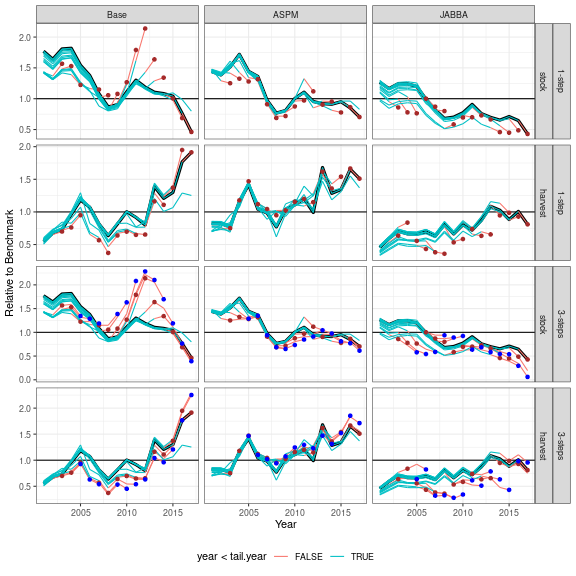
\includegraphics[width=6in]{final-retro-all-1.png}
\caption{Retrospective analysis for the three models, points indicate the terminal years, and the think line the assessment using all the data.}
\label{fig:retro}
\end{figure*}

\begin{figure*}[htbp]
\centering
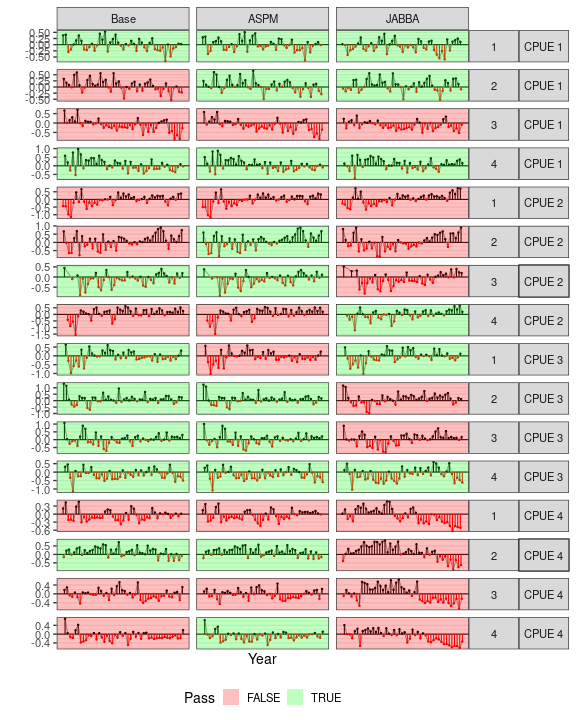
\includegraphics[width=6in]{final-cpue-residual-runs-1.png}
\caption{Residual runs tests for fits to the three models; green background indicates series where runs tests are passed.}
\label{fig:runs}
\end{figure*}

\begin{figure*}[htbp]
\centering
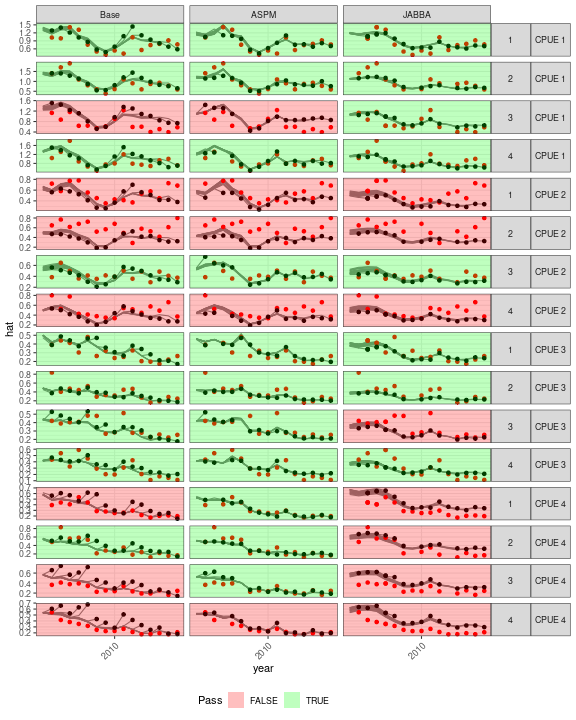
\includegraphics[width=6in]{final-hy-plot-1.png}
\caption{Hindcasts for one step ahead predictions, red dots are the observed CPUE values and lines are the fits with terminal hincast year indicated by a point.}
\label{fig:hy}
\end{figure*}

\begin{figure*}[htbp]
\centering
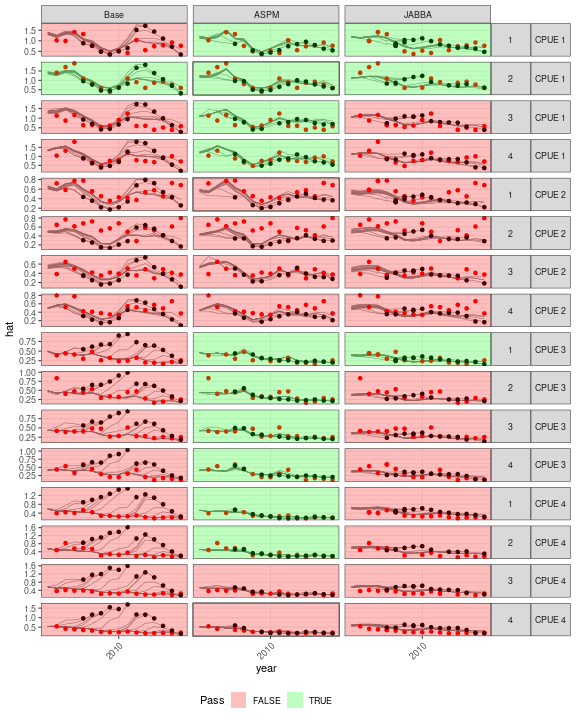
\includegraphics[width=6in]{final-hy3-plot-1.png}
\caption{Hindcasts for three step ahead predictions, red dots are the observed CPUE values and lines are the fits with terminal hincast year indicated by a point.}
\label{fig:hy3}
\end{figure*}


%\begin{figure*}[htbp]
%\centering
%\includegraphics[width=6in]{final-cpue-prediction-runs-1.png}
%\caption{Runs tests for one step ahead residuals.}
%\label{fig:runshat}
%\end{figure*}

\begin{figure*}[htbp]
\centering
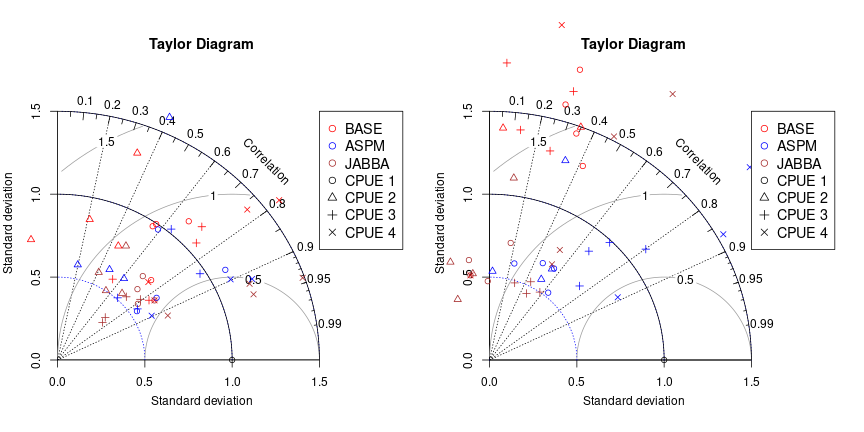
\includegraphics[width=6in]{final-taylor-hy-1-1.png}
\caption{Taylor diagram for one and three year ahead predictions,  summarising the similarity between the observed time series of CPUEs and the predicted relative stock abundance. Each point quantifies how closely predictions match observations, the angle indicates the correlation, the centred root-mean-square error difference between the predicted and observed patterns is proportional to the distance to the point on the x and the contours around this point indicate the RMSE values; the standard deviations of the predictions are proportional to the radial distance from the origin, scaled so the observed pattern has a value of 1. The open circle corresponds to a series which is identical to the reference series. The colours correspond to the model and shape to the survey.)}
\label{fig:td}
\end{figure*}


\end{document}
